\documentclass[twoside,a4paper]{report}
\usepackage{natbib}           % Bibtex
\usepackage{amssymb}
\usepackage{amsmath}
\usepackage{array}            % Eqnarray etc.
\usepackage{graphicx}         % Figures
\DeclareGraphicsExtensions{.jpg,.jpeg,.pdf,.png,.mps,.eps,.ps}
\usepackage[colorlinks=true,raiselinks=true,linkcolor=blue,citecolor=blue,urlcolor=blue]{hyperref}
\usepackage[center]{caption}
\usepackage{setspace}
\setlength{\parindent}{0in}     % Don't indent paragraph
\linespread{1.0}                % Increase linespread
\usepackage{anysize}            % To decrease margins
\marginsize{3.5cm}{3.5cm}{3.5cm}{3cm}
\usepackage{supertabular} 	% Tabellen op meerdere pagina's
\usepackage{tabularx}

\title{Lagrangian Particle Tracking Module in UCLA-LES
}
\author{Bart van Stratum, Thijs Heus and Axel Seifert}

% -------------------------------------------------
\begin{document}


% -------------------------------------------------
\maketitle

\pagenumbering{roman}
% -------------------------------------------------
\tableofcontents
% -------------------------------------------------

% -------------------------------------------------
\chapter{Introduction}
% -------------------------------------------------

Over the past decades, the combination of large-eddy simulation (LES) and Lagrangian particle dispersion models (LPDM) has been employed to study a wide range of topics, ranging from (e.g.) dispersion characteristics in the dry convective boundary layer \citep{mason1992,weil2004,dosio2005,verzijlbergh2009} to mixing processes and entrainment in shallow convection and stratocumulus \citep{heus2008,yamaguchi2012}. In short, LPDM's track the position in space and time of massless particles in the LES domain, driven by the resolved velocities obtained from the Eulerian grid. Compared to conventional (Eulerian) statistics, Lagrangian statistics provide additional information on the history of a particle: it's previous location, state, etc. This provides new possibilities for analyzing processes in LES, e.g. \textit{'where did the air inside this cloud originate? Where and when was this parcel of air entrained in, or detrained from the mixed-layer?'}. By tracking the position of virtual particles, answering these kind of questions becomes possible.\newline

This manual describes the Lagrangian Particle Tracking Module (LPTM) as implemented in UCLA-LES. It starts in chapter 2 with a short guideline for working with the LPTM, describing the required input, output and potential pitfalls of working with the code. Chapter 3 provides a theoretical background of Lagrangian particle tracking, including a reflection on certain implementation choices (e.g. interpolation scheme, use of sub-grid schemes). Chapter 4 describes the implementation in UCLA-LES, with the aim of simplifying the understanding of the module's code. In chapter 5 both a validation of the LPTM, and some additional examples are provided.

\setcounter{page}{1}
\pagenumbering{arabic}

% -------------------------------------------------
\chapter{Using UCLA-LES with the LPTM}
\label{chap:usingLPTM}
% -------------------------------------------------

This chapter acts as a starting point for working with the LPTM in UCLA-LES. Importantly, it starts by outlining the limitations of the module. Secondly, it describes the  
options that can be supplied through the namelist, the required input files, the NetCDF output files and tools available for post-processing of the results.\newline

% -------------------------------------------------
\section{Limitations \& known problems}
% -------------------------------------------------

The LPTM as implemented in UCLA-LES has a number of potential pitfalls; limitations which could result in unphysical or non-logical results:

\begin{itemize}
 \item One of the great advantages of using Lagrangian particles is gaining additional knowledge of the history of a parcel of air. However, within the LPTM implementation in UCLA-LES and when using \textit{lrandsurf}=.true., particles are randomized near the surface in order to maintain a spatially homogeneous distribution (section \ref{sec:subgrid}). As this basically 'breaks' the history of the parcels, special attention should be given to particles that have visited the surface.
 \item For most purposes it is useful to initiate the LPTM with a uniform particle distribution. However, as UCLA-LES uses the anelastic LES equations, turbulence mixes the particles towards a distribution proportional to the base state density ($\rho_0$). To prevent the particle distribution from deviating from its initial distribution, it is therefore best to start the LPTM with a density weighted particle field (see section \ref{sec:req_input}).
 \item The online statistics (section \ref{sec:output}, \texttt{expnme.particlestat.nc}) are based on sampling of particle data over vertical height bins, defined by the vertical grid spacing of the LES experiment. The usability is strongly limited when (i) the vertical particle spacing differs from the grid spacing and/or (ii) a vertical level contains little or no particles. Note that this only influences the online statistics, it doesn't influence the working of the LPTM and should still produce valid results when post-processing the raw particle output (\texttt{expnme.particles.xxxxyyyy.nc}).
\end{itemize}


\clearpage
% ------------------------------------------
\section{Namelist options}
\label{sec:namelist}

\begin{center}
	\tablefirsthead{
        \multicolumn{1}{c}{Option} & \multicolumn{1}{c}{Default} & \multicolumn{1}{c}{Possible values} & \multicolumn{1}{c}{Description} & \multicolumn{1}{c}{Unit}\\
        \hline &&&&\\
  }
  \tablehead{
        \multicolumn{5}{l}{\small \it Continued from previous page}\\
        \multicolumn{5}{c}{}\\
        \multicolumn{1}{c}{Option} & \multicolumn{1}{c}{Default} & \multicolumn{1}{c}{Possible values} & \multicolumn{1}{c}{Description} & \multicolumn{1}{c}{Unit}\\
        \hline &&&&\\
  }
  \tabletail{
        &&&&\\\hline
        \multicolumn{5}{c}{}\\
        \multicolumn{5}{r}{\small \it Continued on next page}\\
  }
  \tablelasttail{
        &&&&\\\hline
  }
\begin{supertabular}{|l|p{1.2cm}|p{3cm}|p{5.0cm}|l|}
  \textit{lpartic}	& .false.	& $x\in\{\text{.false.},\text{.true.}\}$	& Switch for the LPTM					& -\\
  \textit{lpartsurf}	& .false.	& $x\in\{\text{.false.},\text{.true.}\}$	& Switch for randomizing the surface layer		& -\\
  \textit{lpartsgs}	& .false.	& $x\in\{\text{.false.},\text{.true.}\}$	& Switch for the sub-grid scheme				& -\\
  \textit{lpartstat}	& .false.	& $x\in\{\text{.false.},\text{.true.}\}$	& Switch for bin-averaged profile statistics 		& -\\
  \textit{lpartdump}	& .false.	& $x\in\{\text{.false.},\text{.true.}\}$	& Switch for raw particle dump				& -\\
  \textit{lpartdumpui}	& .false.	& $x\in\{\text{.false.},\text{.true.}\}$	& Switch for adding velocities to dump 			& -\\
  \textit{lpartdumpth}	& .false.	& $x\in\{\text{.false.},\text{.true.}\}$	& Switch for adding potential temperature to dump	& -\\
  \textit{lpartdumpmr}	& .false.	& $x\in\{\text{.false.},\text{.true.}\}$	& Switch for adding moisture mixing ratios to dump	& -\\
  \textit{frqpartdump}	& 3600		& $x \in \mathbb{R}, \quad x>0$			& Time interval for writing particle dump		& s\\
\end{supertabular}
\end{center}

% ------------------------------------------
\section{Required input}
\label{sec:req_input}

The LPTM requires both the initial position and release time of each individual particle, supplied to UCLA-LES in ASCII-format in a file named \texttt{partstartpos}. The motivation for using ASCII files (instead of binary or NetCDF files) is that this simplifies the manual creation of \texttt{partstartpos} for debugging or testing purposes. The first line should always contain the total number of particles, followed by the release time (in seconds) and position (in meters) of each particle on a separate line. A Python script is provided to create a uniformly distributed particle field, written to \texttt{partstartpos}. With the correct surface pressure, base state potential temperature and base state pressure provided, the script creates a density weighted distribution, consistent with the base state density in UCLA-LES. The Python script is located in \texttt{UCLALESROOT/misc/LPTM/make\_particles.py} and can be invoked by calling:

\begin{verbatim}
python make_particles.py
\end{verbatim}

All options (release time and grid characteristics) are hard-coded inside \texttt{make\_particles.py}. Some additional information on Python is provided in appendix \ref{app:python}.

% ------------------------------------------
\section{Output}
\label{sec:output}

The LPTM can produce two sets of output:
\begin{itemize}
 \item 'Raw' particle output (switch \textit{lpartdump}) which by default only contains the position of each particle, written at an interval of dt=\textit{frqpartdump}. In addition to the particle position, the interpolated velocities (switch \textit{lpartdumpui}), liquid water and virtual potential temperature (switch \textit{lpartdumpth}) and the total and cloud water mixing ratios (switch \textit{lpartdumpmr}) can be added. In order to balance the I/O load, all cores write a subset of the particles to \texttt{expnme.particles.xxxxyyyy.nc}. Methods and tools to merge the individual NetCDF files are described in section \ref{sec:postp}.
 \item Vertical profiles (switch \textit{lpartstat}) where the properties of all particles within a certain height bin (defined by the vertical grid spacing) are averaged. These statistics are useful for a fast and simple first validation of the results, e.g. by comparing them to Eulerian statistics. Therefore, the sampling and averaging of these statistics is synchronized with the main statistics module of UCLA-LES (\textit{ssam\_intvl} and \textit{savg\_intvl}) and written to \texttt{expnme.particlestat.nc}.
\end{itemize}

In addition, restart files are created (synchronized with the other restart files of UCLA-LES) which allow a warm start of UCLA-LES with the LPTM.

% ------------------------------------------
\section{Post-processing}
\label{sec:postp}

\subsection{Merging raw output}

A Fortran script (with makefile) to merge the individual NetCDF files is provided in\\ \texttt{UCLALESROOT/misc/LPTM/merge\_particles.f90}. This script can convert the individual files, containing all variables of a subset of particles (output UCLA-LES), to NetCDF files containing the complete record (all particles) of one variable. After compiling, the script can be executed as:

\begin{verbatim}
./merge_particles rico x 8 8
\end{verbatim}

for \texttt{expnme = rico}, variable $x$ and 8 processors in both the x and y direction. To automatically call this script after UCLA-LES is finished, a Python script is provided in \texttt{UCLALESROOT/misc/LPTM/auto\_particlemerge.py}. When placed (together with \texttt{merge\_particles}) in the same directory as the job-script and invoked by adding:

\begin{verbatim}
python auto_particlemerge.py
\end{verbatim}

to the end of the job-script, this script automatically determines the case prefix and number of processors used in the X and Y direction, and creates and submits a serial job for each variable ($x,y,z,u,v,w,t,tv,rt,rl$).

\subsection{Data analysis}

For those who are interested in using Python for post-processing, an example script is provided in \texttt{UCLALESROOT/misc/LPTM/process\_particles.py} which demonstrates  the use of Python (with some inline \texttt{C++}) for post-processing. The use of inline \texttt{C++} allows for optimization of a number of loops, resulting in a performance comparable (but not equal) to e.g. Fortran or other non-interpreted languages. 

% ------------------------------------------
\chapter{Theoretical description LPTM}
\label{chap:theory}

\section{Lagrangian particle tracking}

In short, the LPTM tracks the position (and properties) of virtual massless particles in the LES domain. The displacement of each particle is determined by the Lagrangian velocity $u_{i,L}$ \citep[e.g.][hereafter W04]{weil2004}: 

\begin{equation}
 \frac{\partial x_{i,p}}{\partial t} = u_{i,L}; \:\:\:\: u_{i,L} = \widetilde{u}_{i,p} + u_{i}^{sgs},
 \label{eq:xip}
\end{equation}

where $x_{i,p}$ is the position of the particle, $\widetilde{u}_{i,p}$ is the resolved or filtered velocity from LES, interpolated to the position of the particle and $u_{i}^{sgs}$ is a contribution of sub-grid processes to the Lagrangian velocity (section \ref{sec:subgrid}). At each time step the resolved velocity is interpolated from the staggered LES grid to the location of each particle (section \ref{sec:interpolation}) and subsequently the displacement is integrated to obtain the new position of the particle (section \ref{sec:integration}). 

\section{Spatial interpolation}
\label{sec:interpolation}

To provide $\widetilde{u}_{i,p}$, interpolation from the staggered LES grid to particle position is needed. Like in \cite{heus2008}, a simple trilinear interpolation is implemented in UCLA-LES:

\begin{eqnarray}
 \widetilde{u}_{i,p} = (1-\delta x)(1-\delta y)(1-\delta z)    u_{i,1}    &+&               \\
                          \delta x \: (1-\delta y)(1-\delta z) u_{i,2}    &+&               \nonumber \\
                          \delta x \: \delta y \: (1-\delta z) u_{i,3}    &+&               \nonumber \\
                      (1-\delta x) \: \delta y \: (1-\delta z) u_{i,4}    &+&               \nonumber \\
                      (1-\delta x)(1-\delta y) \: \delta z \:  u_{i,5}    &+&               \nonumber \\
                      \delta x \: (1-\delta y) \: \delta z \:  u_{i,6}    &+&               \nonumber \\
                      \delta x \: \delta y \: \delta z \:      u_{i,7}    &+&               \nonumber \\
                      (1-\delta x) \: \delta y \: \delta z \:  u_{i,8},                     \nonumber \\
\end{eqnarray}

where $u_{i,\chi}$ refers to the velocity points surrounding the particle and $\delta x_i$ is the relative displacement ($0 \geq \delta x_i > 1 $) as shown in Fig. \ref{fig:trilinear}. Despite the simplicity of the linear interpolation, it provided satisfactory results in the work of e.g. \cite{heus2008,verzijlbergh2009}. Moreover, it is a computationally cheap method requiring only the eight surrounding velocity points. Other methods like e.g. tricubic interpolation \citep[see][for a supposedly efficient method]{lekien2005} or the fifth-order Lagrange polynomial interpolation in the LPTM of \cite{yamaguchi2012} require additional information; more grid points, velocity derivatives, etc. 

\begin{figure}
  \begin{center}
    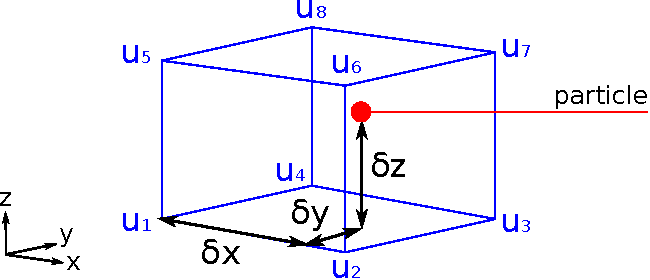
\includegraphics[width=0.40\textwidth]{figures_LPTM/trilinear.pdf}
    \caption{Coordinates trilinear interpolation}
    \label{fig:trilinear}       % Give a unique label
  \end{center}
\end{figure}

\section{Integration scheme}
\label{sec:integration}

A third-order Runge-Kutta integration scheme is used to numerically integrate Eq. \ref{eq:xip}, similar to the time solver in UCLA-LES:

\begin{eqnarray}
 x^{t*}_{i,p}   &=& x^{t}_{i,p}   + \alpha_1 u^t_{i,L}    \Delta t                                        \\
 x^{t**}_{i,p}  &=& x^{t*}_{i,p}  + \alpha_2 u^t_{i,L}    \Delta t  + \beta_2 u^{t*}_{i,L}  \Delta t      \nonumber \\
 x^{t+1}_{i,p}  &=& x^{t**}_{i,p} + \alpha_2 u^{t*}_{i,L} \Delta t  + \beta_2 u^{t**}_{i,L} \Delta t,     \nonumber \\
\end{eqnarray}

where $^{t*}$ and $^{t**}$ denote the intermediate Runge-Kutta steps, $u_{i,L}$ is the Lagrangian velocity (Eq. \ref{eq:xip}) and $\alpha_j = \{\frac{8}{15},\frac{-17}{60},\frac{3}{4}\}$, $\beta_j = \{0,\frac{-15}{12},\frac{-15}{12}\}$. The particle algorithm is called at the beginning of each RK3 step of UCLA-LES, such that the velocities used to determine the particle displacement match those used to calculate other tendencies in the time solver. 

%\begin{center}
%\setlength{\unitlength}{1mm}
%\begin{picture}(50,25)
%  \put(0,18){$x_t$} 
%  \put(5,19){\vector(1, 0){5}}
%  \put(12,18){$x_t^*$} 
%  \put(17,19){\vector(1, 0){5}}
%  \put(24,18){$x_t^{**}$} 
%  \put(29,19){\vector(1, 0){5}}
%  \put(36,18){$x_{t+1}$} 

%  \put(0,10){$u_t^i$} 
%  \put(5,11){\vector(1, 0){5}}
%  \put(12,10){$u_t^{i*}$} 
%  \put(17,11){\vector(1, 0){5}}
%  \put(24,10){$u_t^{i**}$} 
%  \put(29,11){\vector(1, 0){5}}
%  \put(36,10){$u_{t+1}^i$} 

%  \multiput(7,3)(0,2){10}{\line(0,1){1}}
%  \multiput(31,3)(0,2){10}{\line(0,1){1}}
%  \put(15,4){$RK3$} 
%\end{picture}
%\end{center}

\section{Representation sub-grid processes}
\label{sec:subgrid}

Although LES resolves a large fraction of the turbulent flow, Lagrangian dispersion models mostly include an additional representation for sub-grid-scale processes (Eq. \ref{eq:xip}). For example, \cite{lamb1978} used a stochastic (Monte Carlo) model, relating the magnitude of the sub-grid displacement to the sub-grid-scale TKE. \cite{mason1992} used a similar approach, imposing a random sub-grid velocity near the surface, based on a Gaussian velocity distribution with a standard deviation related to a prescribed eddy diffusivity profile. A more advanced approach was coined by W04 with a prognostic equation for the sub-grid-scale velocity, again based on the unresolved TKE. However, other studies neglected the sub-grid-scale processes altogether as it provided only little or no improvement \citep{Gopal2000,dosio2005,yamaguchi2012}.

\subsection{The need for a sub-grid model?}

As shown by \cite[][Fig. A1]{heus2008}, the most important artifact of not including a sub-grid model is the accumulation of particles near the surface. This can be explained by the vertical velocity distribution in the CBL; typically positively skewed \citep[e.g.][]{Stull1988} with large slowly subsiding areas, locally compensated by strong updrafts. This slowly transports particles towards the surface layer, until being transported upwards again by an updraft. In an ideal  divergence free flow, the updraft should cause horizontal convergence towards the root of the updraft, transporting particles to it and thus compensating for the rapid removal of particles near the surface. Unfortunately, as turbulence is by definition poorly resolved in this part of LES, the compensation is limited, resulting in a horizontally nonuniform particle distribution with an excess of particles near the surface.

\subsection{Sub-grid model Weil (W04)}

The model of W04 solves the before mentioned problem \citep{heus2008} by adding a sub-grid component to the Lagrangian velocity. However, one of the assumptions underlying their derivation is that the sub-grid-scale turbulence is isotropic. While this assumption might hold in the bulk in the CBL, it is questionable near the surface or other regions dominated by sub-grid-scale processes. Also, most studies using the model of W04 use it in combination with the prognostic TKE sub-grid model of Deardorff. Testing of the model in UCLA-LES (using the Smagorinsky sub-grid model), with the sub-grid TKE calculated as described by \cite{stevens1999}, partially solved the accumulation of particles near the surface, but introduced unwanted particle displacements in other regions (see chapter \ref{chap:examples}). Nonetheless, the model of W04 is available in UCLA-LES.\newline

The contribution of sub-grid processes is determined using a prognostic equation:

\begin{equation}
  du'_i = - \left(\frac{f_s \: C_0 \: \epsilon \: u'_i}{2 \sigma^2_{sgs}}\right)dt 
          + \frac{1}{2} \left( \frac{1}{\sigma^2_{sgs}} \frac{d\sigma^2_{sgs}}{dt} u'_i + \frac{\partial \sigma^2_{sgs}}{\partial x_i}\right) dt
          + (f_s \: C_0 \: \epsilon)^{\frac{1}{2}} \: d\xi,
\label{eq:duisgs}
\end{equation}

where $u_i$ denotes the sub-grid velocity and $f_s$ the relative sub-grid contribution of the total variance:

\begin{equation}
  f_s = \frac{\sigma^2_{sgs}}{\sigma^2_{sgs} + \sigma^2_{res}},
\label{eq:fs}
\end{equation}

$C_0$ is a constant, $\epsilon$ the dissipation rate of turbulence, $\sigma^2_{sgs}$ the sub-grid velocity variance and $d\xi$ is a component of a Gaussian white noise. 
In W04, $f_s$ is calculated using slab-averaged variances. Although this might be a useful and valid simplification for a dry CBL, local differences in $f_s$ are to be expected in cases with (i.a.) shallow convection. Hard-coded in \texttt{particles.f90} is the possibility to switch between the local or global calculation (with respectively \textit{lfsloc=.true.} or \textit{.false.}). For isotropic turbulence, $\sigma^2_{sgs} = \frac{2}{3}e$ and with $\epsilon = \frac{C_\epsilon}{\lambda}e^{3/2}$, equation \ref{eq:duisgs} is implemented in UCLA-LES as:

\begin{equation}
  du'_i = \underbrace{-\frac{3}{4} f_s \: C_0 \: u'_i \: \frac{C_\epsilon}{\lambda} \: \left(\frac{3}{2} \sigma^2_{sgs}\right)^\frac{1}{2} \: dt}_{(I) \: dissipation}
          \underbrace{+\frac{1}{2} \left( \frac{1}{e} \frac{de}{dt} u'_i + \frac{2}{3}\frac{\partial e}{\partial x_i}\right) dt}_{(II) \: relation \: sgs-tke}
          \underbrace{+\left(f_s \: C_0 \: \frac{C_\epsilon}{\lambda}\left[\frac{3}{2}\sigma^2_{sgs}\right]^{\frac{3}{2}}\right)^\frac{1}{2} \: d\xi}_{(III) \: random \: fluctuation}
\label{eq:duisgs_uclales}
\end{equation}

Term I represents the dissipation of the sub-grid velocity and should, in theory, only decrease the absolute value of $u'$ to zero. However, the integration becomes unstable when $e$ approaches zero, causing an excessive growth of term II (containing $1/e$). This can influence term I, causing it to overshoot the decrease of the absolute value of $u'$, thus causing a sign change in $u'$. To prevent this from happening, both term I and II are limited such that their individual contribution to $du'$ cannot change the sign of $u'$. The physical explanation of this limitation of term II is similar to that of term I. Term II relates the tendency of $u'$ to the time and spatial change in $e$. Again, this term is allowed to increase or decrease the absolute value of $u'$, but not change its sign. \newline

Eq. \ref{eq:duisgs} is integrated at the beginning of each RK3 cycle and subsequently used in each RK3 step in Eq. \ref{eq:xip}, i.e. the same sub-grid velocities are used for all intermediate RK3 steps. 

%The limitation in UCLA-LES is implemented as:
%\[
% du' = 
%  \begin{cases} 
%   du'     & \text{if } \mathrm{sign(u'+du) = sign(u')} \\
%   -u'     & \text{else } 
%  \end{cases}
%\]

\subsection{Alternative solution}

As a more direct solution to the accumulation of particles near the surface, the inhomogeneous particle distribution can be homogenized by giving each particle near the surface a random (horizontal) position within the domain. The randomization allows for a more effective removal of particles from the near-surface layer, and has proved to be a reliable (i.e. relatively insensitive to the used grid spacing) solution. In addition, this method is computationally less expensive than the method of W04 (section \ref{sec:overhead}).\newline

For highly parallel experiments it is necessary to randomize the particles over the entire domain, as a single sub-domain (the column handled by one process) might largely consist of an up- or downdraft. In the LPTM, the particles are globally randomized when \textit{lpartsurf=.true.} and the particles reside in the lowest grid level of the domain.

\subsection{Considerations when using a sub-grid representation}
\label{sec:rec_subgrid}

Both solutions perform satisfactory (see the validation and comparison in chapter \ref{chap:examples}), however:

\begin{enumerate}
 \item Like the LPTM in DALES \citep{heus2010}, the model of W04 performs the best with $f_s$ fixed at one. In the current version, $f_s$ is therefore harcoded to one using the switch \texttt{fixedfs} in \texttt{particles.f90}.
 \item The computational overhead of W04 is quite large (section \ref{sec:overhead}) and more optimization might be needed. 
 \item The solution using surface randomization performs well and has a negligible computational overhead (section \ref{sec:overhead}), but puts a serious constraint on the use of Lagrangian particles near the surface.   
\end{enumerate}


\chapter{Implementation in UCLA-LES}

\section{Data management}

The main difference between Eulerian and Lagrangian statistics from a coding point of view is that where all Eulerian grid-points reside at fixed spatial positions, the Lagrangian particles are free to move around. In a parallel environment, this results in a constant traffic of particles, moving from processor core to core. As this constantly changes the amount of particles per core or process, it is inconvenient to use arrays for the storage of the particle position, velocity, etc. To prevent this problem, each particle is stored in a data structure, coupled together in a linked list. The idea behind this is shown in Fig. \ref{fig:linked_list}. Each particle record contains, in additions to its data, also a reference (pointer to the memory address of) its previous and next particle. When a particle (here record ``B'') is removed or moved to another processor, only the pointers need to be changed to again create a closed list. 

\begin{figure}[h]
  \begin{center}
    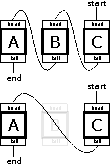
\includegraphics[width=0.2\textwidth]{figures_LPTM/linked_list.pdf}
    \caption{Daisy chaining of the particle records}
    \label{fig:linked_list}       % Give a unique label
  \end{center}
\end{figure}

\section{Domain \& coordinate system}

\subsection{Coordinate system}

Throughout the entire module, the location and velocities of the particles are defined in grid coordinates, i.e. its location and displacement relative to a grid with a grid spacing of $\Delta x, \Delta y, \Delta z = \{1,1,1\}$ (Fig. \ref{fig:grid_coord}). In the horizontal plane, the ghost cells are incorporated in the coordinate system, with the actual domain (or sub-domain in a parallel environment) starting at x,y = 3. When a particle passes the horizontal boundaries of the domain (x,y $<$ 3 or x,y $\geq$ 6 for Fig. \ref{fig:grid_coord}) it is handed over to the next processor. In a non-parallel environment, cyclic boundaries are used. The transformation from coordinates in meters is directly performed during the initialization, and reverted only when statistics or output needs to be written. \newline

\subsection{Boundary conditions}

At the land surface and model top, reflective boundaries are used, i.e. all particles which end at a height $\delta z$ below (above) the surface (model top) are displaced to a height $\delta z$ above (below) the surface (model top) (Fig. \ref{fig:grid_coord}). For particles near the surface ($z<1.5$) the horizontal velocity components are interpolated to zero at $z=1$. 

\begin{figure}[h]
  \begin{center}
    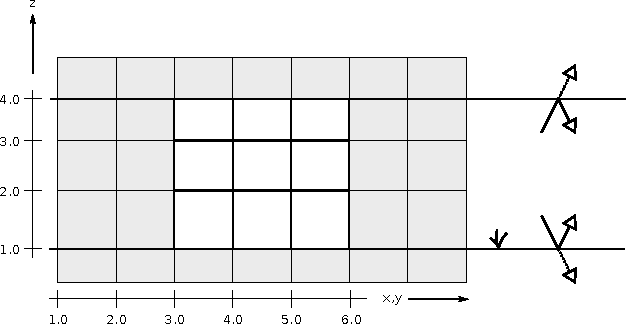
\includegraphics[width=0.8\textwidth]{figures_LPTM/grid_coord.pdf}
    \caption{Use of grid coordinates, gray cells denote the ghost cells}
    \label{fig:grid_coord}       % Give a unique label
  \end{center}
\end{figure}

\section{Overview routines in modparticles.f90}

Fig. \ref{fig:routines_modparticles} shows the main LPTM routines called from init.f90 and step.f90. The different colors refer to the namelist flags (section \ref{sec:namelist}), i.e. these routines are only called when the corresponding flag is set to true. The core of the LPTM consists of 3 subroutines which initialize and finalize the particles (\texttt{init\_particles()}, from partstartpos or the restart file, and \texttt{exit\_particles()}), and \texttt{particles()} which is called each RK3 step and is the main driver of the LPTM. In its most bare form, \texttt{particles()} does the interpolation (\texttt{ui3d()}, \texttt{vi3d()}, \texttt{wi3d()}), integration (\texttt{rk3()}) and boundary checking and communication (\texttt{checkbound()}, \texttt{partcomm()}). All other subroutines are optional and handle statistics, the raw particle dumps, and subgrid representations.

\begin{figure}[h]
  \begin{center}
    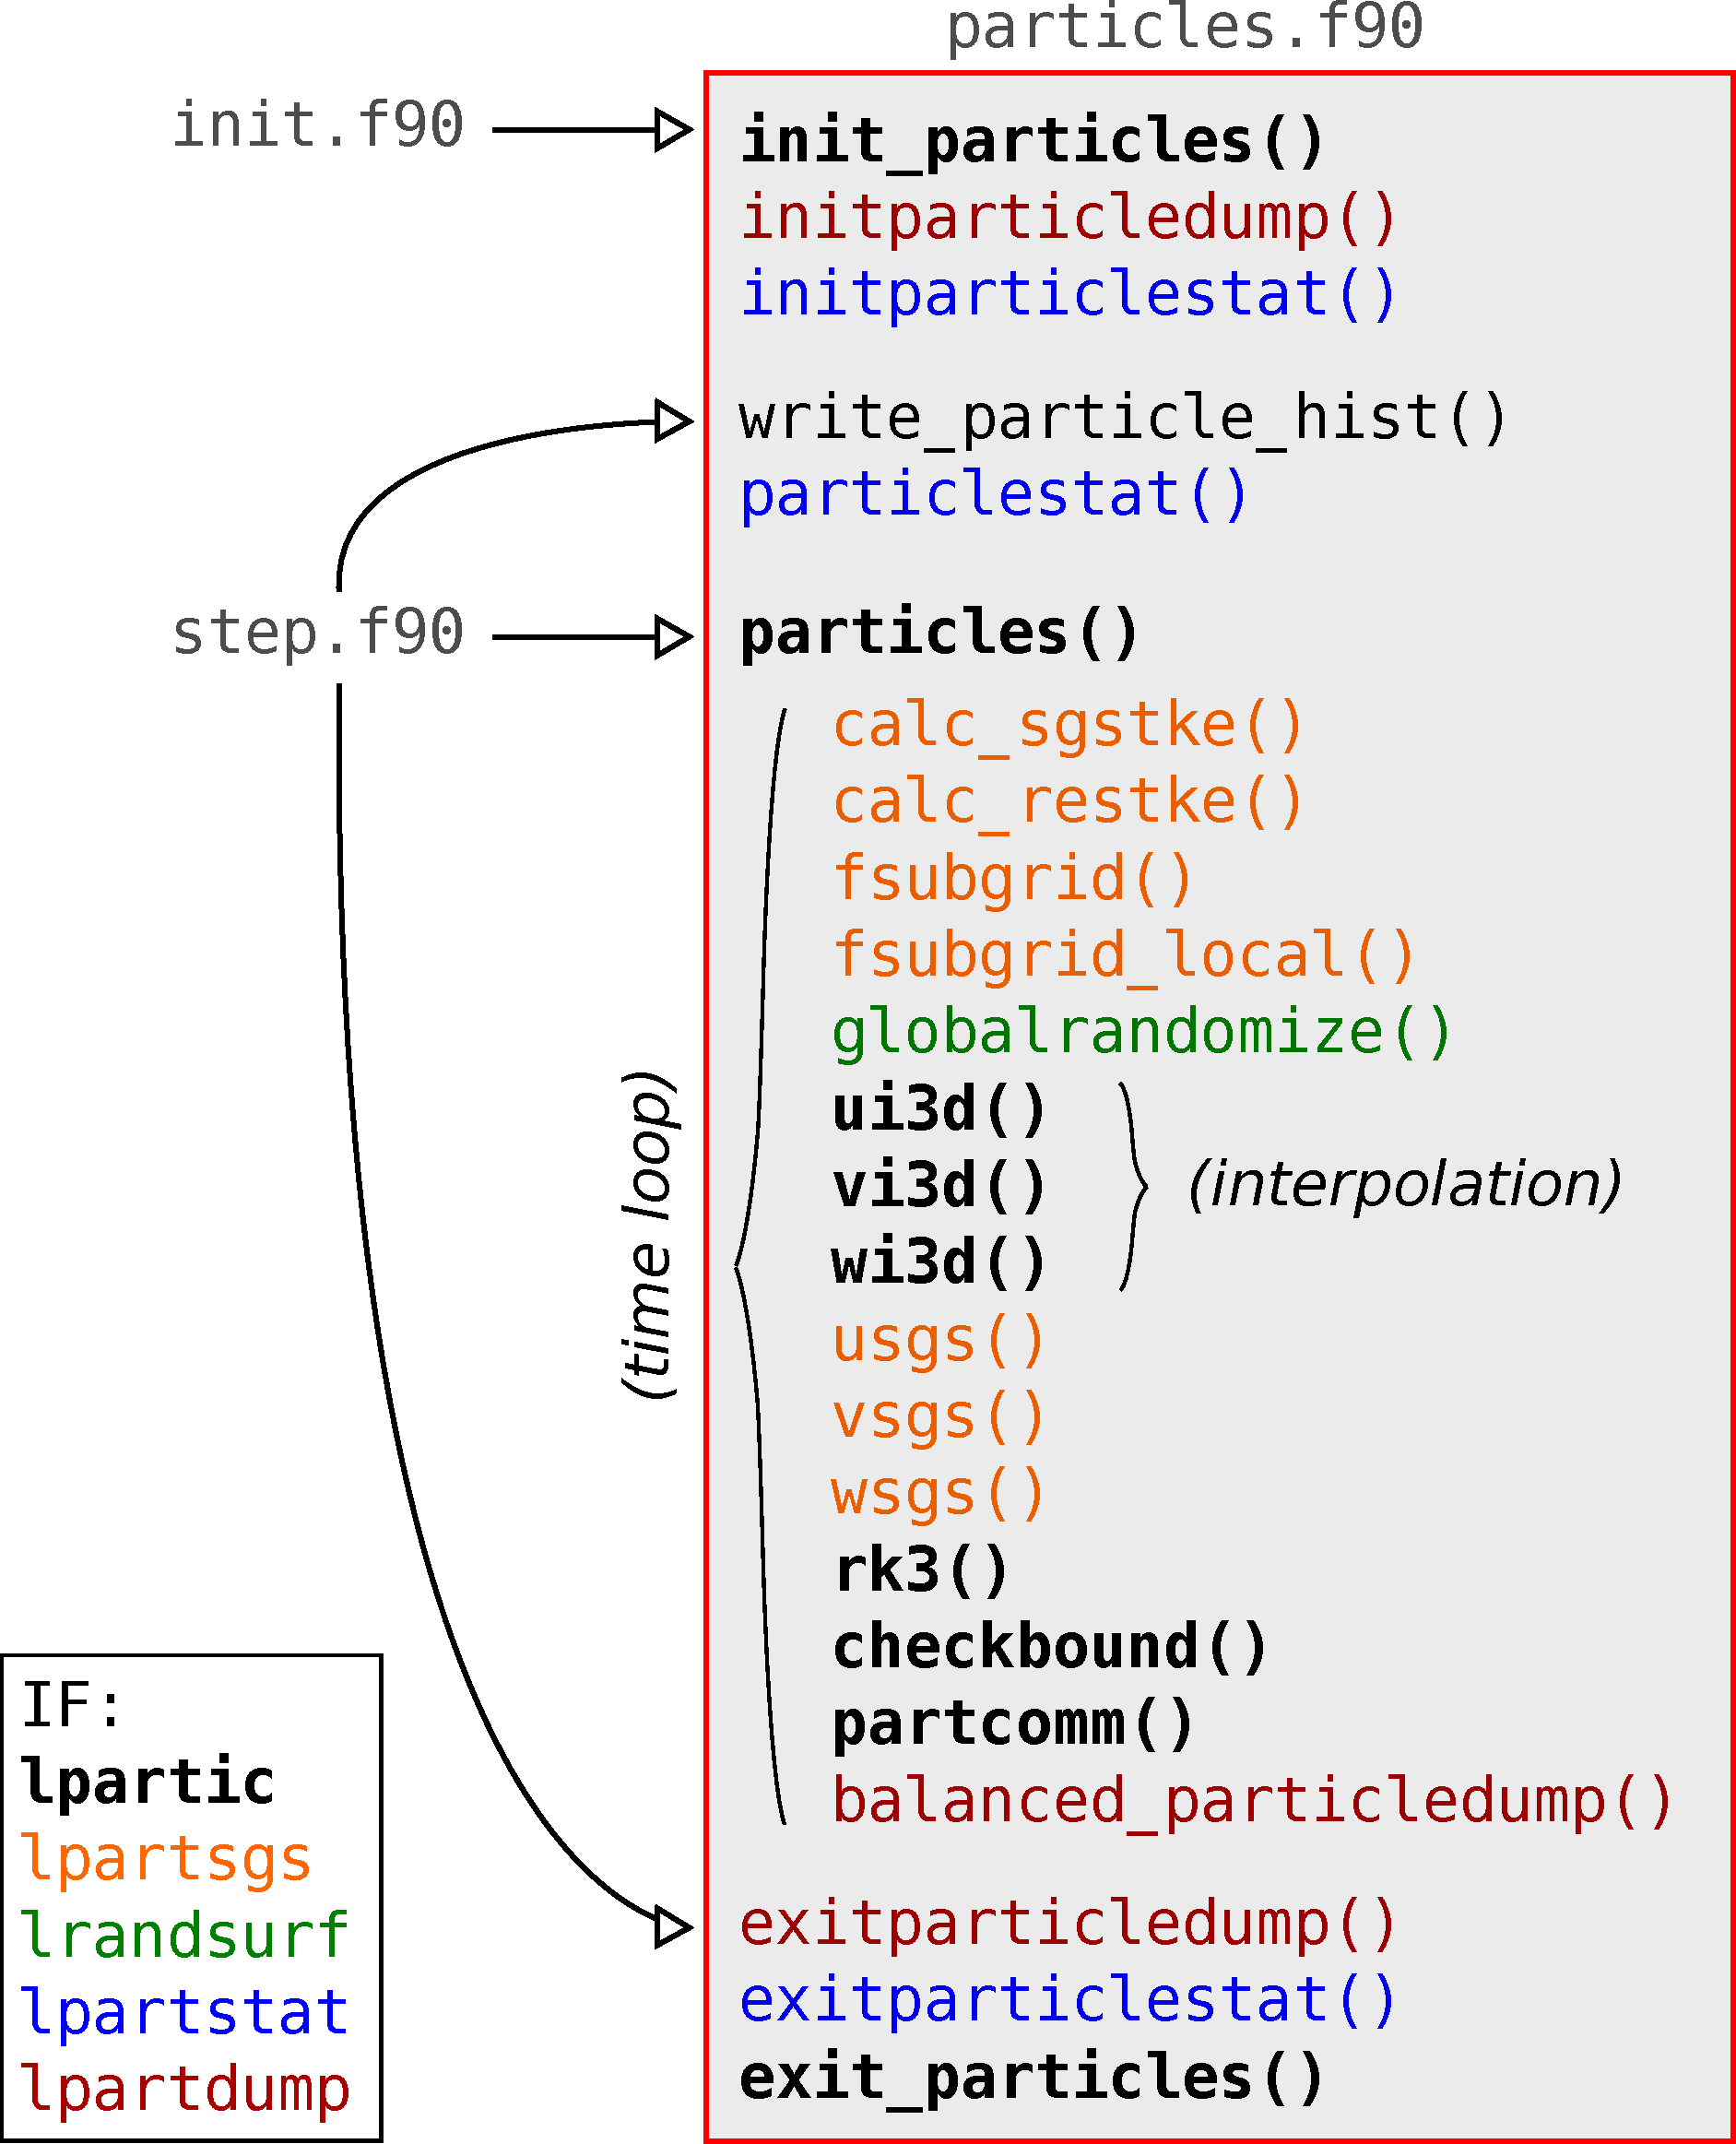
\includegraphics[width=0.6\textwidth]{figures_LPTM/routines.pdf}
    \caption{Overview of the main particle routines called by init.f90 and step.f90}
    \label{fig:routines_modparticles}       % Give a unique label
  \end{center}
\end{figure}

\section{Computational overhead LPTM}
\label{sec:overhead}

To determine the computational overhead of the LPTM, short experiments (900s integration time) for the RICO case \citep{vanZanten2011} with 128x128x160 grid cells at 25x25x25m grid spacing and $\sim$2.27 million particles have been performed. All tests were executed on 2 complete nodes on Blizzard (64 cores) to add some inter-node communication to the setup. Compared to a simulation with no particles (reference), the bare particle code (with no sub-grid scheme, surface randomization or output) increased the wall-clock time by 31\%. The additional overhead of both the surface randomization and particle dumps (every 60s) was negligible (an additional increase in wall-clock time of 0.2\%). The largest bottleneck is the sub-grid scheme of W04, where the wall-clock time is increased by 57\% compared to the reference case. As this inefficiency was not reported about the LPTM in DALES \citep{heus2010}, more optimization of this part of the code might be needed.   

% ------------------------------------------
\chapter{Examples}
\label{chap:examples}

The goal of this final chapter is twofold: (1) to validate the results of the LPTM and (2) to demonstrate some of the possibilities that Lagrangian particles provide.

\section{Validation LPTM: RICO case}

As described by \cite{heus2008}, there are two important criteria for the validation of Lagrangian statistics in LES:

\begin{enumerate}
 \item[(1)] A homogeneous particle distribution should stay homogeneous in an incompressible flow.
 \item[(2)] For a sufficiently large amount of particles, the Lagrangian and Eulerian statistics should converge.
\end{enumerate}

In this first example, both criteria are tested for the RICO case \citep{vanZanten2011} in a 3200m x 3200m x 4000m domain using a grid spacing of 25m in all directions ($nxp = nyp = 128, \: nzp = 160$). A total of ~2.25 million particles were released after 1 hour, and tracked continuously for the next 11 hours. As a comparison, Fig. \ref{fig:exa_subgrid_dales} shows the results of criterion (1) as presented by \cite{heus2008}. Note that there is a significant difference in the particle integration time between their study (4 hours) and these results presented here (11 hours).\newline

To test the various options in the UCLA-LES LPTM, a number of simulations were performed:

\begin{itemize}
 \item[-] \textit{(bare)} No representation for sub-grid processes (\textit{lrandsurf}=false, \textit{lpartsgs}=false)
 \item[-] \textit{(Weil)} Sub-grid model Weil with a bulk value for $f_s$ (\textit{lpartsgs}=true)
 \item[-] \textit{(Weil $f_s$=1)} Sub-grid model Weil with $f_s$=1 (\textit{lpartsgs}=true)
 \item[-] \textit{(surface rand())} Surface randomization (\textit{lrandsurf}=true)
\end{itemize}

\begin{figure}[h]
  \begin{center}
    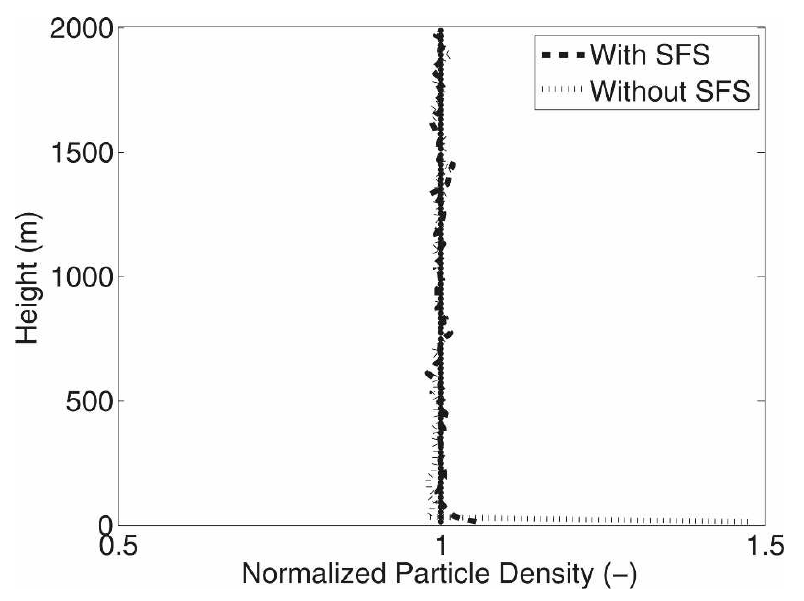
\includegraphics[width=0.5\textwidth]{figures_LPTM/pdensity_dales.png}
    \caption{Validation of the criterion (1) in DALES (BOMEX case), reprinted from \cite{heus2008}. ``With SFS'' denotes the experiment with the model of W04.}
    \label{fig:exa_subgrid_dales}       % Give a unique label
  \end{center}
\end{figure}

\begin{figure}[hb!]
  \begin{center}
    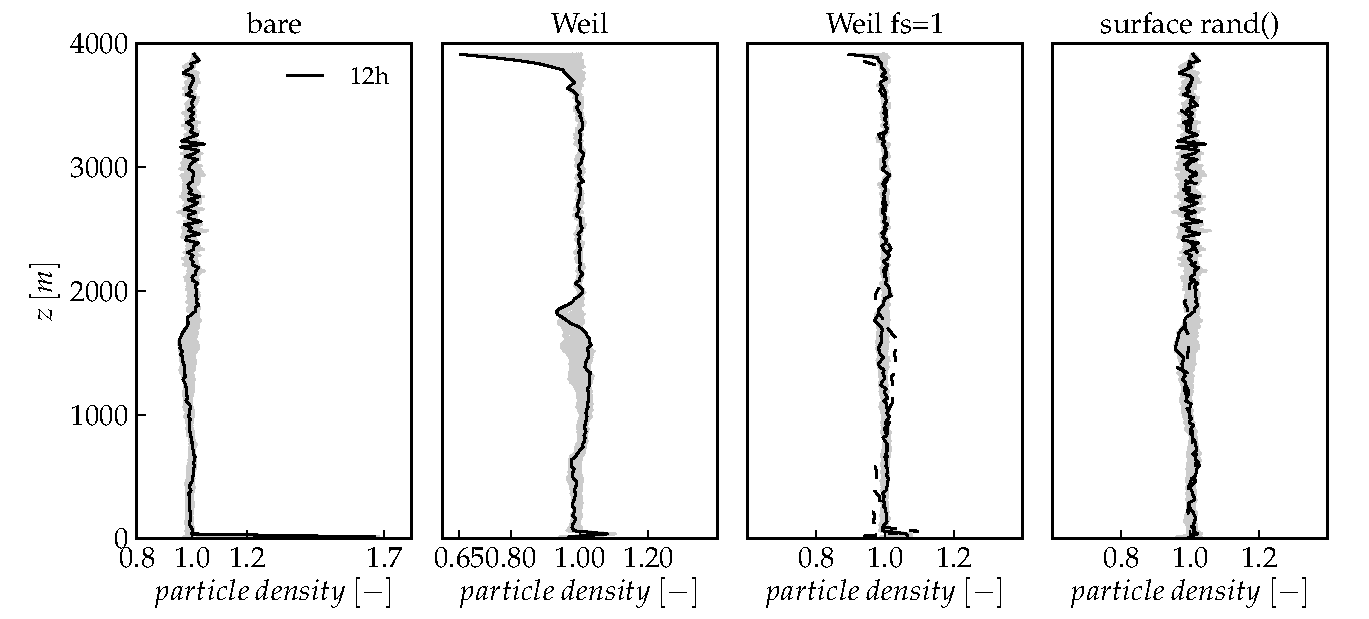
\includegraphics[width=1.0\textwidth]{figures_LPTM/rico_comp_subgrid.pdf}
    \caption{Validation of the criterion (1) with no sub-grid representation \textit{(bare)}, W04's model \textit{(Weil)}, \textit{(Weil $f_s$=1)} and surface randomization \textit{(surface rand())}. The dashed lines are the result of a second experiment at a lower resolution, the gray shaded area indicates the spread in the results between 1-12h. All data is sampled at the end of the simulation, i.e at t=12h.}
    \label{fig:exa_subgrid}       % Give a unique label
  \end{center}
\end{figure}

Note that \textit{(Weil $f_s$=1)} is not a default option and requires hard-coded changes in particles.f90.\newline

The first case \textit{(bare)} demonstrates the accumulation of particles near the surface, as explained in section \ref{sec:subgrid}. This process is non-stationary, i.e. the accumulation of particles continues and showed no sign of reaching an equilibrium in longer experiments. The second case \textit{(Weil)} partially solves this problem, but introduces a particle drift in areas with a gradient in $f_s$ (near-surface, inversion / transition layer and model top, where the latter is caused by the sponge layer). This problem is removed by fixing $f_s$ at one \textit{(Weil $f_s$=1)}, although this is a somewhat artificial solution as it requires the assumption in Weil's model that no turbulence is resolved (Eq. \ref{eq:fs}). The solution using the surface randomization \textit{(surface rand())} performs slightly better near the surface compared to \textit{(Weil $f_s$=1)}, and slightly worse near the cloud top (here at $\sim$1800m), but overall performs satisfactory. For the last two cases, a second experiment at a lower resolution (100 x 100 x 40m, dashed lines) was performed to test the dependency on the grid spacing and amount of unresolved turbulence. In \textit{(Weil $f_s$=1)} this slightly increases the accumulation near the surface to 10\%. The experiment using surface randomization shows no dependency on the grid spacing. \newline

\begin{figure}[h]
  \begin{center}
    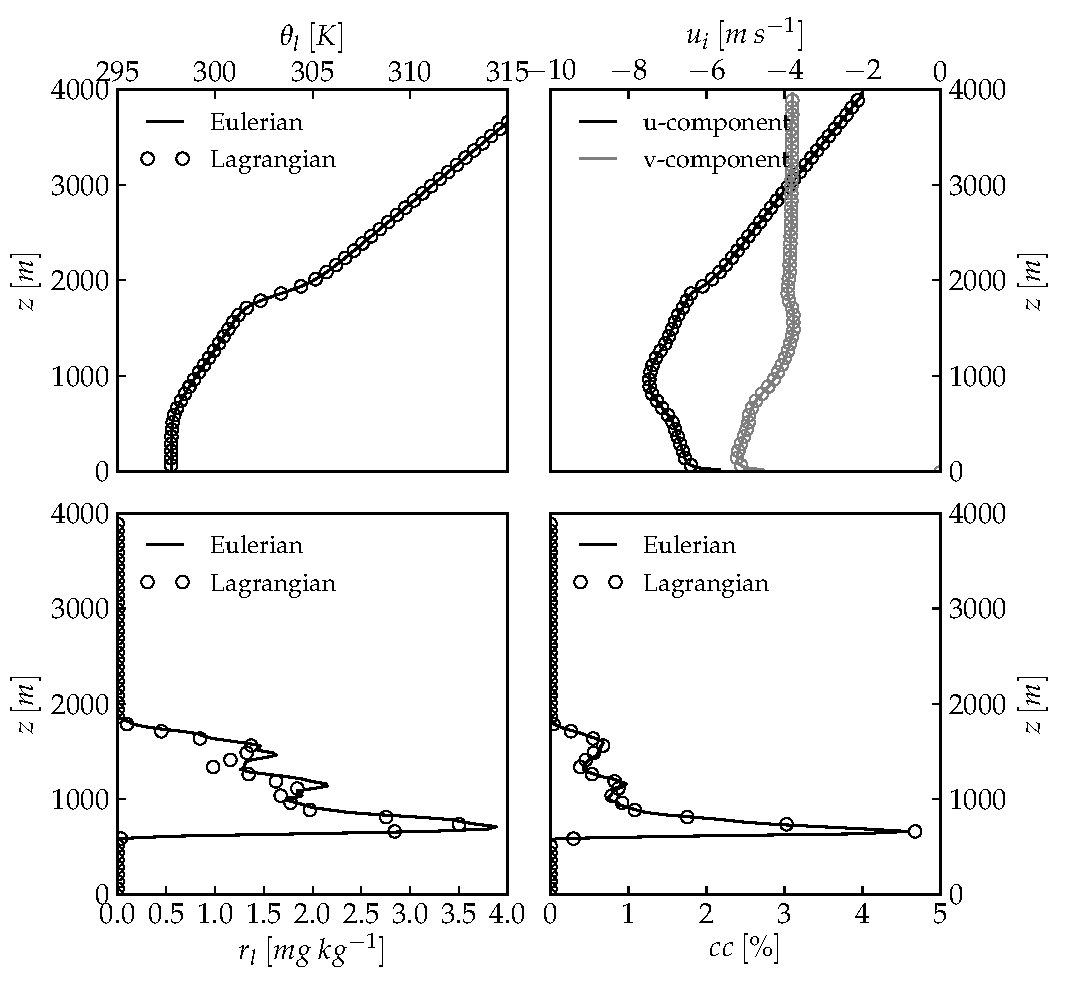
\includegraphics[width=0.85\textwidth]{figures_LPTM/rico_eul_vs_lagr.pdf}
    \caption{Comparison between the Lagrangian and Eulerian statistics for the liquid water potential temperatur ($\theta_l$), horizontal velocity components, liquid water mixing ratio ($r_l$) and cloud cover.}
    \label{fig:exa_eul_vs_lagr}       % Give a unique label
  \end{center}
\end{figure}

To test criterion (2), the online statistics (section \ref{sec:output}) from case \textit{surface rand()} are compared to the Eulerian statistics for a number of variables in Fig. \ref{fig:exa_eul_vs_lagr}. When comparing these statistics, a distinction has to be made between quantities that are conserved and therefore can be directly interpolated to the particle position (e.g. the liquid water potential temperature, $\theta_l$, or velocities) and quantities that are calculated at the particle position (e.g. liquid water mixing ratio, $r_l$, or cloud cover). The latter is necessary because of the non-linearity in Clausius-Clapeyron, making it more accurate to calculate saturation at the particle position using interpolated values for $\theta_l$, $r_t$ and pressure than to simply interpolate $r_l$ from the LES grid. \newline

Fig. \ref{fig:exa_eul_vs_lagr}a,b show the comparison for $\theta_l$ and the two horizontal velocity components. For all three variables, there is a close match between the Eulerian and Lagrangian statistics, indicating that the interpolation scheme (section \ref{sec:interpolation}) is working correctly. For the liquid water mixing ratio and cloud cover in Fig. \ref{fig:exa_eul_vs_lagr}c,d a small discrepancy between the Eulerian and Lagrangian statistics is found. However, in a test (not shown) where the Lagrangian particles were fixed at the scalar position in the Eulerian grid, both statistics again converged, indicating that the thermodynamic calculations at the particle location are working correctly. \newline

Finally, the velocity variances for both statistics are compared in Fig. \ref{fig:exa_variances}. Again there is a satisfactory match between the Eulerian and Lagrangian statistics, although the Lagrangian variances are slightly underestimated. As shown in \cite{heus2008}, this is the result of first interpolating the velocities to the particle position before squaring them, instead of squaring the velocities before interpolation.\newline

In summary, the LPTM in UCLA-LES is working correctly, with two possible solutions to prevent the accumulation of particles near the surface. 

\begin{figure}[h]
  \begin{center}
    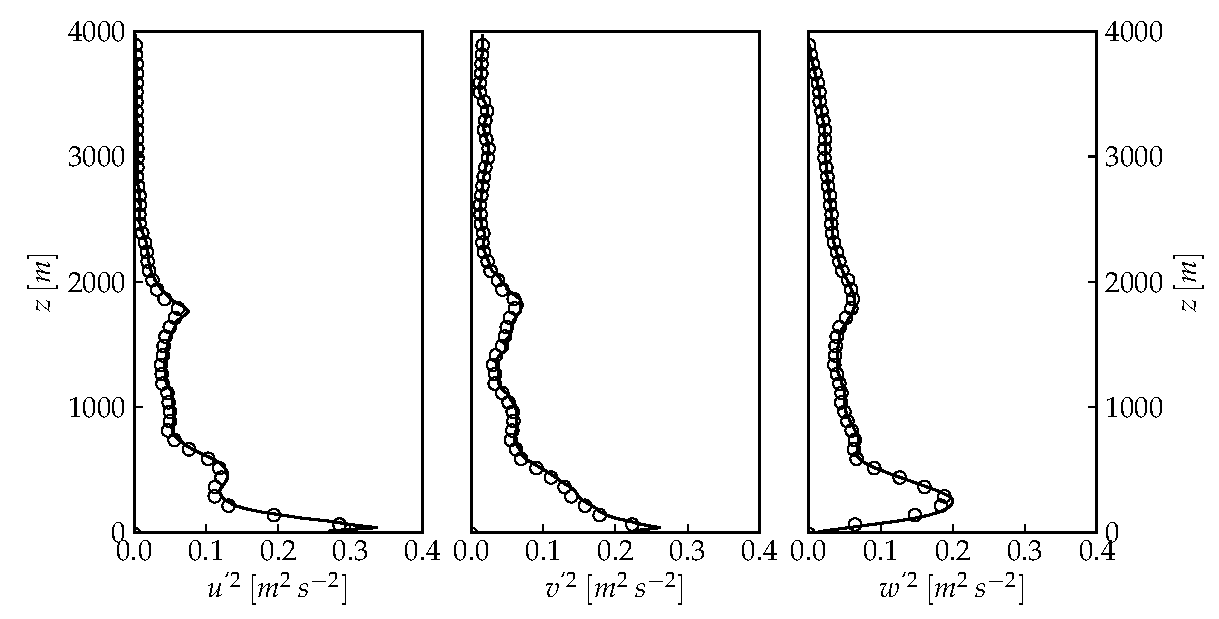
\includegraphics[width=0.9\textwidth]{figures_LPTM/rico_variances.pdf}
    \caption{Comparison between the Lagriangian and Eulerian velocity variances.}
    \label{fig:exa_variances}       % Give a unique label
  \end{center}
\end{figure}

% ------------------------------------------
%\chapter*{Appendix A: Using Python}
\appendix
\chapter{Using Python}
\label{app:python}
%\addcontentsline{toc}{chapter}{Appendix A: Using Python}

Python is fairly similar to e.g. Matlab: an easy to learn, high level programming language. Also, with some additional libraries, the possibilities for use in scientific computation and analysis are very similar. The main difference is however that Python is free and by default available on most Linux or OS X systems. Scripts can be invoked from the command-line using:

\begin{verbatim}
python script.py
\end{verbatim}

To access some useful additional libraries (\textit{Numpy} for using numerical arrays or matrices, \textit{Scipy} for advanced math, signal processing, statistics and more and \textit{Matplotlib} for scientific quality plotting), the module python/2.7-ve0 (MPI desktops) or python/2.7.0 (Lizard) first needs to be loaded.\newline

Explaining Python goes beyond the scope of this manual and is unnecessary as there are some very good tutorials or manuals available online, e.g.:

\begin{itemize}
\item General manual of Python: \url{http://docs.python.org/tutorial/}
\item Scipy (scientific Python): \url{http://www.scipy.org/Getting_Started/}
\item Numpy (numerical Python): \url{http://www.scipy.org/Tentative_NumPy_Tutorial/}
\item Matplotlib (scientific plotting): \url{http://matplotlib.sourceforge.net/}
\end{itemize}





\addcontentsline{toc}{chapter}{\bf References}
%\renewcommand\chapterheadstartvskip{\vspace*{-2\baselineskip}}
\setlength\bibsep{5pt}
\bibliographystyle{agsm} 
\bibliography{./references_LPTM}

\end{document}
